\documentclass[11pt]{article}

%------------------------------------------------------------------
%------------------------------------------------------------------
%------------------------------------------------------------------
% Informació de l'informe

\newcommand{\titol}{
	 Modelado y control cinemático
	 }

\newcommand{\titolcap}{Modelado y control cinemático}

\newcommand{\AlumnoA}{Carlos Mira López}
\newcommand{\AlumnoB}{Nicolás Miró Mira}
\newcommand{\AlumnoC}{Vittorio Alessandro Esposito Ceballos}

\newcommand{\AlumnosPie}{\AlumnoA\ -- \AlumnoB\ -- \AlumnoC}
\newcommand{\Asignatura}{Asignatura}
\newcommand{\CursoTitulacion}{4$.\!^\circ$ curso - Grado en Ingeniería ...}
%https://www.rae.es/dpd/ordinales

\newcommand{\Data}{Octubre de 2022}

%------------------------------------------------------------------
% Configuració de formats i bibliografia


\usepackage[spanish,es-tabla,es-nosectiondot,es-sloppy,es-noshorthands]{babel} 

\usepackage[utf8]{inputenc}
\usepackage{mathtools}
\usepackage{graphicx,xcolor}
\usepackage{tabularx,booktabs}

\usepackage{float}

\floatstyle{plaintop}
%\floatstyle{ruled}
\newfloat{listado}{htbp}{lol}
\floatname{listado}{Listado}

\usepackage[tableposition=top]{caption}
\renewcommand{\captionlabelfont}{\bfseries\small}
\renewcommand{\captionfont}{\small\itshape}
%\captionsetup[table]{position=above}

\usepackage{enumitem}
\setlist{leftmargin=1.25cm}

\renewcommand{\labelenumi}{\arabic{enumi})}
\renewcommand{\labelenumii}{\alph{enumii})}

% ---------------------------------------------------------------------
% Document electrònic

\usepackage[ 
    colorlinks,
    linkcolor = blue,
    urlcolor = blue,
    citecolor = blue,
    ]{hyperref}

% ---------------------------------------------------------------------
% Configuració de pàgina

\usepackage{geometry}
\geometry{
    a4paper, 
    twoside = false,
    hmargin = {2.5cm,2.5cm},
    vmargin = {1cm,1cm},
    headsep = 1.0cm,
    footskip = 1.5cm,
    includehead, includefoot
    }
        
% ---------------------------------------------------------------------
% Unitats del sistema internacional

\usepackage{siunitx}
\sisetup{
    output-decimal-marker = {,},
    % per-mode = symbol,
    }
    
% ---------------------------------------------------------------------
% Capçaleres i peus de pàgina

\usepackage{fancyhdr}
\pagestyle{fancy}

\usepackage{lastpage}

\fancyhead{} 
% \fancyhead[L]{\footnotesize \sffamily \titolcap}
% \fancyhead[R]{\footnotesize \sffamily \nouppercase \leftmark}
\fancyfoot{} 
% \fancyfoot[R]{\sffamily\footnotesize\thepage/\pageref*{LastPage}}
\ifundef{\AlumnosPie}
	{
		\fancyfoot[L]{\sffamily\footnotesize Se debe configurar el nombre de los alumnos que aparece en el pie}
	}
	{
		\fancyfoot[L]{\sffamily\footnotesize\AlumnosPie}
	}
\renewcommand{\headrulewidth}{0.4pt}
\renewcommand{\footrulewidth}{0.4pt}

% ---------------------------------------------------------------------
% Confiuració de la bibliografia

\usepackage[
	url = false,
	style = apa,
	%style = ieee,
	hyperref = true,
	backref = true,
	]{biblatex}

\usepackage{csquotes}

% ---------------------------------------------------------------------
% On estan les figures? 

\graphicspath{
    {./figuras/}
    {./logos/}
    }

% ---------------------------------------------------------------------
% Informació de portada

\usepackage{xifthen}

\newboolean{LogoUPV}
\newboolean{LogoAlcoi}

\ifundef{\AlumnoB}{\newcommand{\AlumnoB}{}}{}
\ifundef{\AlumnoC}{\newcommand{\AlumnoC}{}}{}

\title{\Huge\bfseries%
	\vspace*{-1cm}
    \ifLogoAlcoi
	   
\includegraphics[width=5cm]{UPV_Campus_Alcoi}\\
    \else
        
\includegraphics[width=5cm]{UPV_horitzontal_color}\\
    \fi
    \vspace*{6cm}
    \titol
    \vspace*{3.5cm}
    ~
    }
    
\author{
    \AlumnoA\\[1ex]
    \AlumnoB\\[1ex]
	\AlumnoC\\[3.5cm]
  	\textbf{\Asignatura}\\[2ex]
  	\textbf{\CursoTitulacion}
    }
    
\date{\Data}

% ---------------------------------------------------------------------
% Format de paràgraf

\parindent = 0cm
\parskip = 2ex
\partopsep = -1ex

% ---------------------------------------------------------------------
% Control de línies orfes i vídues

\clubpenalty = 10000
\widowpenalty = 10000
\displaywidowpenalty = 10000

% ---------------------------------------------------------------------
% Comandaments personalitzats

\usepackage{xspace}

\newcommand{\matlab}{{\textsc{Matlab}}\xspace}
\newcommand{\simulink}{\textit{Simulink}\xspace}


% ---------------------------------------------------------------------
% Fi
\usepackage{listings}

\definecolor{Paper}{HTML}{F5F5F5}

% ---------------------------------------------------------------------
% ---------------------------------------------------------------------
% Matlab

\lstset{
	language = Matlab,
	basicstyle = \ttfamily\footnotesize,         
	identifierstyle = ,           
	commentstyle = \color[rgb]{0,.5,0},
	stringstyle = \color[rgb]{.7,.2,.7},
	tabsize = 4,
	showstringspaces = false,
	frame = single,
	rulecolor = \color[rgb]{0.3,0.3,0.3},
	framerule = 0.2pt,
	framesep = 9pt,
	xleftmargin = 9pt,
	xrightmargin = 9pt,		
	backgroundcolor = \color{Paper},
	morekeywords = {},
	keywordstyle = \color{blue},
	}


% ---------------------------------------------------------------------
% ---------------------------------------------------------------------
% C

%\lstset{
%	language = C,
%	basicstyle = \ttfamily\small,         
%	identifierstyle = ,           
%	commentstyle = \color[rgb]{.4,.4,.4},%\itshape,
%	stringstyle = \color[rgb]{0,.5,0},
%	tabsize = 4,
%	morekeywords = {},
%	keywordstyle = \color{blue},	
%	frame=single,
%	framesep = 9pt,
%	xleftmargin = 24pt,
%	xrightmargin = 16pt,		
%	backgroundcolor = \color{Paper},
%	numbers = left,                    
%	numbersep = 16pt,                   
%	numberstyle = \scriptsize\color[rgb]{.4,.4,.4}, 
%	rulecolor = \color{black},         
%	showspaces = false,                
%	showstringspaces = false,          
%	showtabs = false,        
%	}

% ---------------------------------------------------------------------
% ---------------------------------------------------------------------

\lstset{literate= % Para poder usar acentos
  {á}{{\'a}}1 {é}{{\'e}}1 {í}{{\'i}}1 {ó}{{\'o}}1 {ú}{{\'u}}1
  {Á}{{\'A}}1 {É}{{\'E}}1 {Í}{{\'I}}1 {Ó}{{\'O}}1 {Ú}{{\'U}}1
  {à}{{\`a}}1 {è}{{\`e}}1 {ì}{{\`i}}1 {ò}{{\`o}}1 {ù}{{\`u}}1
  {À}{{\`A}}1 {È}{{\'E}}1 {Ì}{{\`I}}1 {Ò}{{\`O}}1 {Ù}{{\`U}}1
  {ä}{{\"a}}1 {ë}{{\"e}}1 {ï}{{\"i}}1 {ö}{{\"o}}1 {ü}{{\"u}}1
  {Ä}{{\"A}}1 {Ë}{{\"E}}1 {Ï}{{\"I}}1 {Ö}{{\"O}}1 {Ü}{{\"U}}1
  {â}{{\^a}}1 {ê}{{\^e}}1 {î}{{\^i}}1 {ô}{{\^o}}1 {û}{{\^u}}1
  {Â}{{\^A}}1 {Ê}{{\^E}}1 {Î}{{\^I}}1 {Ô}{{\^O}}1 {Û}{{\^U}}1
  {Ã}{{\~A}}1 {ã}{{\~a}}1 {Õ}{{\~O}}1 {õ}{{\~o}}1
}

% Si vols utilitzar un tipus de lletra semblant a Arial, descomenta les dos línies següents:
% \usepackage{cmbright}
% \usepackage[OT1]{fontenc}

\bibliography{./configuraciones/referencias}

%------------------------------------------------------------------
% Logo:

\setboolean{LogoUPV}{false}
\setboolean{LogoAlcoi}{true}

%------------------------------------------------------------------
%------------------------------------------------------------------
%------------------------------------------------------------------

\begin{document}

% -------------------------------------
% -------------------------------------


\renewcommand{\itemautorefname}{punto}
\renewcommand{\sectionautorefname}{sección}
\renewcommand{\subsectionautorefname}{subsección}
\renewcommand{\subsubsectionautorefname}{subsección}
\renewcommand{\appendixautorefname}{apéndice}
\renewcommand{\figureautorefname}{figura}
\renewcommand{\tableautorefname}{tabla}

\renewcommand{\indexname}{Índice alfabético}
\renewcommand{\bibname}{Bibliograf\'{\i}a}
\renewcommand{\contentsname}{Índice general}
\renewcommand{\abstractname}{Resumen}	

\def\listadoautorefname{listado}

% Per a les ecuacions en una línia
\abovedisplayshortskip = -1.0ex plus 0ex minus 0.25ex
\belowdisplayshortskip = 2.0ex plus 1ex minus 0.0ex

% Per a les equacions en varies línies
\abovedisplayskip = -1.0ex plus 0ex minus 0.25ex
\belowdisplayskip = 2.0ex plus 1ex minus 0.0ex

\begin{titlepage}
    \maketitle
    \thispagestyle{empty}
\end{titlepage}

\renewcommand{\thepage}{\Roman{page}}
\fancyfoot[R]{\sffamily\footnotesize\thepage}
\fancyhead{} 

\renewcommand{\headrulewidth}{0.0pt}

\setcounter{page}{1}

{
\footnotesize
\parskip=1ex

\tableofcontents

\clearpage



}

\clearpage

\renewcommand{\thepage}{\arabic{page}}
\fancyfoot[R]{\sffamily\footnotesize\thepage/\pageref*{LastPage}}
\setcounter{page}{1}

\fancyhead[L]{\footnotesize \sffamily \titolcap}
\fancyhead[R]{\footnotesize \sffamily \nouppercase \leftmark}

\renewcommand{\headrulewidth}{0.4pt} % No eliminar!!!

% -------------------------------------
% -------------------------------------


%------------------------------------------------------------------
%------------------------------------------------------------------
% Resumen

%------------------------------------------------------------------
%------------------------------------------------------------------

\section{Introducción}
\label{sec:introduccion}
En este proyecto se diseña y construye un robot manipulador de al menos tres grados de libertad, controlado con servomotores y una placa Arduino UNO. El objetivo es que el robot pueda mover sus articulaciones de manera precisa, calcular la posición del efector final mediante cinemática directa, y determinar los ángulos necesarios para llegar a posiciones deseadas mediante cinemática inversa.
Además, se desarrolla una interfaz de usuario que permite controlar el robot, ver su posición en coordenadas articulares y cartesianas, y enviar comandos de movimiento de forma sencilla.

%------------------------------------------------------------------
%------------------------------------------------------------------

\section{Descripción del diseño mecánico y electrónico}
\label{sec:diseño}
Hemos optado por el diseño y ensamblaje de un robot angular con 3 grados de libertad, los cuales aparecen como una rotación en la base en el eje x, un movimiento horizontal en el eje z con respecto a la base gracias a un rodamiento que hemos implementado y un movimiento en el eje x del codo del robot, también gracias a un rodamiento implementado.




Utilizamos 3 servos, uno bajo la base para realizar el giro, otro alineado con el rodamiento del brazo para llevar a cabo el movimiento y otro alineado con el rodamiento del codo, también para su movimiento. En cuanto al cableado
\begin{figure}[H]
    \centering
    \includegraphics[width=0.6\linewidth]{figuras/imagen_diseño.jpeg}
    \caption{rebot en plenitud}
\end{figure}

Hay varias maneras de definir la posición inicial, nosotros hemos optado por definir una posición conocida como es la [0,0,0], donde la posición del brazo y del codo son horizontales como se muestra en la primera figura, pudiendo calcular así las distancias y facilitar la calibración y el movimiento del robot
%------------------------------------------------------------------
%------------------------------------------------------------------

\section{Modelo matemático}
\label{sec:modelo}


\begin{figure}[H]
    \centering
    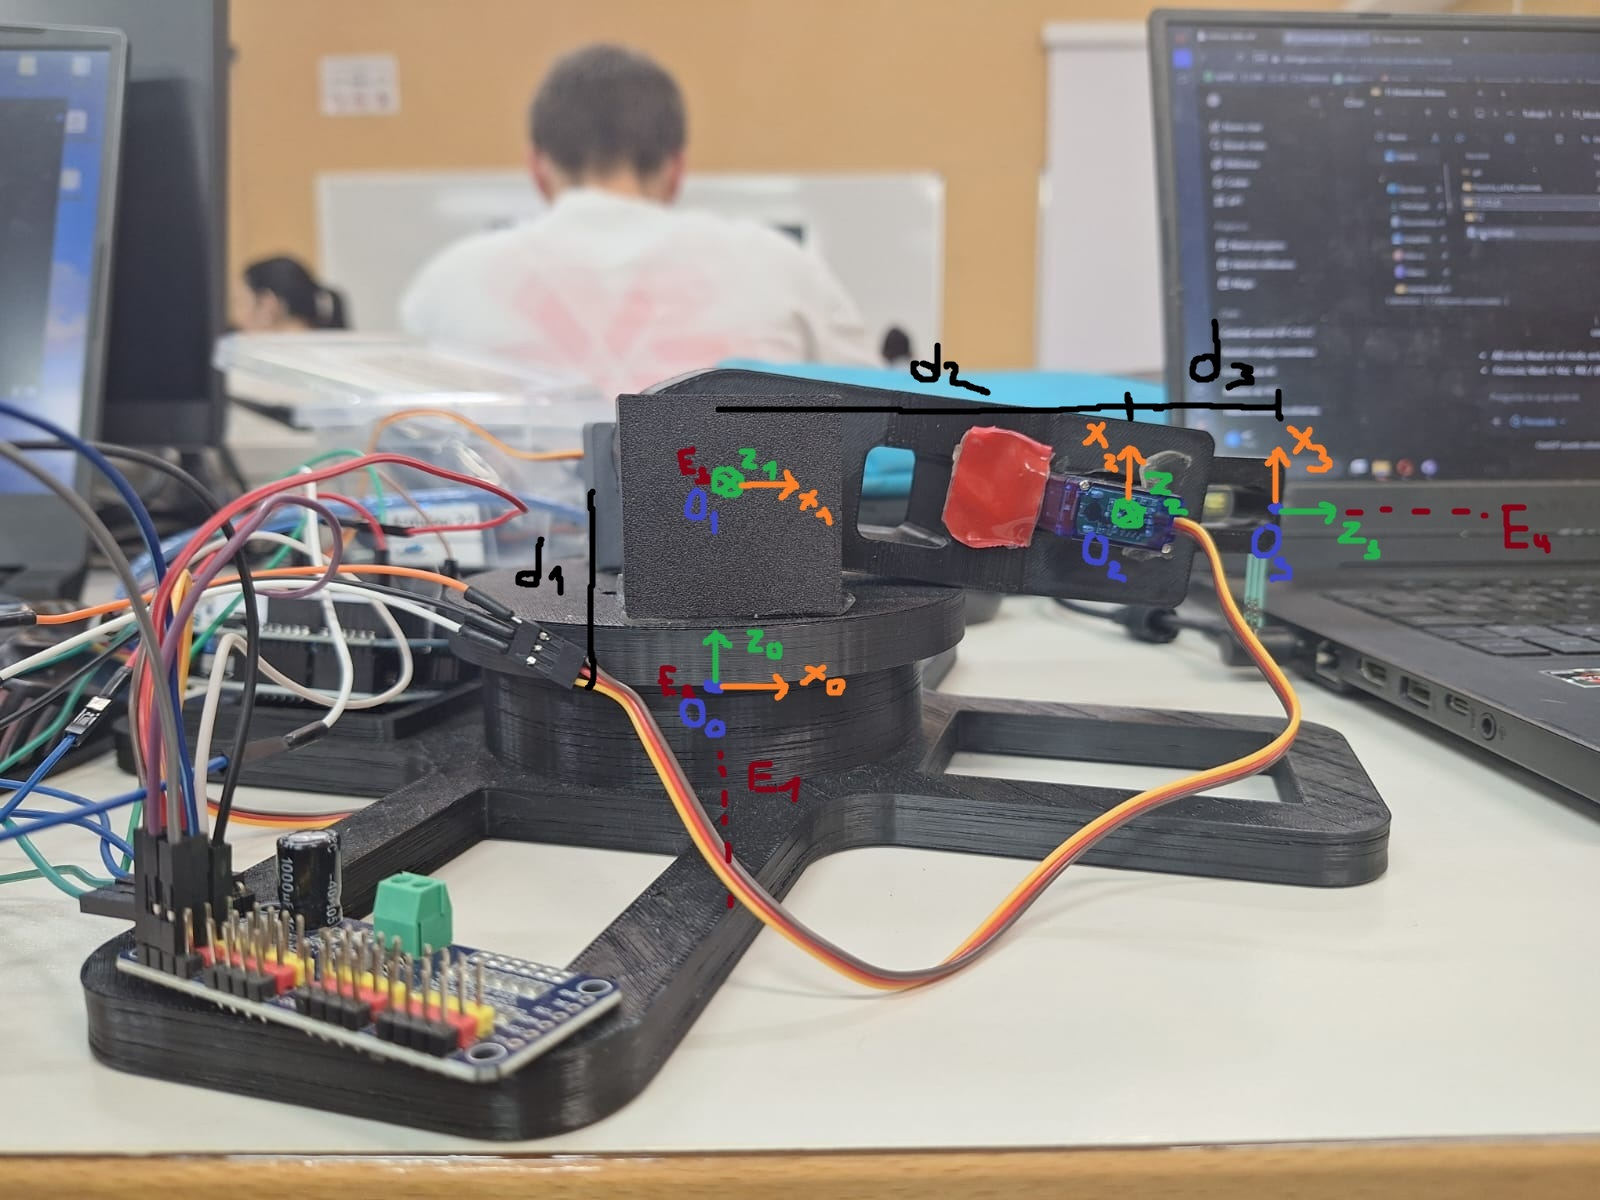
\includegraphics[width=0.8\linewidth]{figuras/imagen_ejes.jpeg}
    \caption{Ejes del robot}
\end{figure}

\[
\begin{array}{c|c|c|c|c}
i & d_i & \theta_i & \alpha_i & a_i \\ \hline
1 & d_1 & 0 & \tfrac{\pi}{2} & 0 \\
2 & 0 & 0 & 0 & d_2 \\
3 & 0 & 0 & 0 & d_3
\end{array}
\]

\subsection{Cinemática directa}
La cinemática directa permite calcular la posición y orientación del efector final (la pinza) a partir de los ángulos y desplazamientos de las articulaciones del robot.

En nuestro caso, el robot tiene 3 grados de libertad:
\begin{itemize}
    \item Rotación en la base (eje X): permite girar todo el brazo alrededor de la base.
    \item Movimiento horizontal en el eje Z: conseguido mediante un rodamiento implementado en la base, que desplaza el brazo a lo largo del eje Z.
    \item Movimiento en el eje X del codo: logrado mediante otro rodamiento, que permite extender o retraer el brazo a lo largo del eje X desde el codo.

\end{itemize}



La posición del efector final $(x,y,z)$ se calcula combinando estas tres transformaciones mediante matrices de transformación homogénea. Multiplicando las matrices correspondientes a cada articulación se obtiene la matriz global $T_0^3$, de la que se extraen las coordenadas de la pinza.

\subsection{Cinemática inversa}
La cinemática inversa permite determinar los ángulos y desplazamientos de las articulaciones necesarios para colocar la pinza en una posición y orientación deseadas.

Para nuestro robot:
\begin{itemize}
    \item Debemos calcular la rotación de la base para orientar el brazo hacia el punto deseado.
    \item Ajustar el desplazamiento horizontal en Z para posicionar la altura correcta.
    \item Ajustar el movimiento en X del codo para llegar a la distancia correcta desde la base.

\end{itemize}


Se deben considerar posibles múltiples soluciones, así como restricciones físicas de los rodillos y límites de las articulaciones. La cinemática inversa asegura que el robot pueda mover su efector a cualquier posición alcanzable dentro de su espacio de trabajo.

%------------------------------------------------------------------
%------------------------------------------------------------------

\section{Código e interfaz}
\label{sec:código}



%------------------------------------------------------------------
\subsection{Código implementado en Arduino}
\begin{lstlisting}
 aqui el codigo
\end{lstlisting}
%------------------------------------------------------------------
\subsection{Interfaz de usuario}
\begin{figure}[H]
    \centering
    \includegraphics[width=0.8\linewidth]{figuras/interfaz.jpeg}
    \caption{Interfaz de usuario}
\end{figure}

Esta es la interfaz de usuario que hemos diseñado, tenemos en primera parte un botón para conectar con el robot, junto con un icono de color que nos indica visualmente si la conección ha sido exitosa o no. debajo de eso elegimos el tipo te cinemática, si la opción está pulsada es cinemática directa, en caso contrario es cinemática inversa; debajo de eso tenemos cajas de texto ajustables para base, brazo y codo del robot, todas junto a iconos de + y -, donde podemos mover paso a paso individualmente cada parte en incrementos o decrementos de 5 grados, acompañado con eso debajo cajas de texto que indican las posición del robot en los ejes X Y y Z.

En cuanto a la parte de la cinemática inversa tenemos cajas de texto donde modificamos el valor de las posiciones de X,Y y Z medidas en milímetros, a lo que después presionamos el botón enviar, lo que mueve el robot a las posiciones elegidas, mostrando en las cajas de abajo el ángulo en la base el brazo y el codo, además del resultado del cálculo de la cinemática inversa
\section{Pruebas y demostración}
\label{sec:pruebas}
En esta sección presentaremos pruebas del funcionamiento del robot



\href{https://www.youtube.com/watch?v=iHJcyHrV9w0}{Link a video de cinemática directa}

\href{https://www.youtube.com/watch?v=igmchIDxLEQ}{Link a video de cinemática inversa}

%------------------------------------------------------------------
%------------------------------------------------------------------

\bibitemsep = 2ex
\bibhang = 2em


%------------------------------------------------------------------
%------------------------------------------------------------------
%------------------------------------------------------------------

\end{document}

%------------------------------------------------------------------
%------------------------------------------------------------------
%------------------------------------------------------------------

